\section{Select \& Fetch}

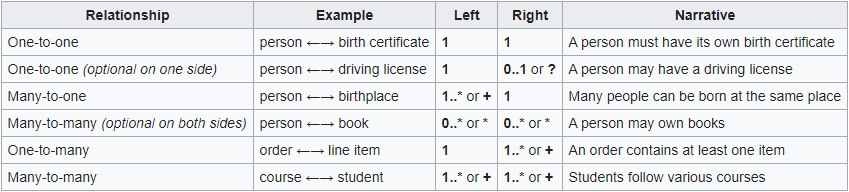
\includegraphics[scale=0.30]{./cardinality.png}

\begin{tiny}
\begin{lstlisting}
SELECT [DISTINCT] select lijst
FROM tabelnaam
[WHERE conditie]
[ORDER BY clausule]
[OFFSET offset ROWS]
[FETCH row limiting clause]
\end{lstlisting}

\begin{lstlisting}
SELECT * FROM employees
WHERE dob
BETWEEN '1-JAN-1980'
AND '31-DEC-1989';
\end{lstlisting}

\begin{lstlisting}
FETCH WITH TIES -- Wanneer je meerdere rijen wilt retourneren die gelijk staan
NULLS FIRST -- Wanneer je NULL waarde als eerst wil tonen
\end{lstlisting}

\begin{lstlisting}
[OFFSET offset ROWS]
FETCH NEXT [row_count]
ROWS [ONLY | WITH TIES]
\end{lstlisting}

\end{tiny}